\documentclass[11pt]{amsbook}
\usepackage{../Ceyhun}
\usepackage{../amsTurkish}
\usepackage{graphicx}
\graphicspath{{images/}}

\title{ceyhun-232}
\author{ceyhun}

\begin{document}

4-boyanırdır. Eğer $ d_0 $ düğümüne bitişik düğümlerin boyanmasında
\textcircled{1}, \textcircled{2}, \textcircled{3}, \textcircled{4}
diye göstereceğimiz 4 ayrı renk de kullanılmamışsa, $ d_0 $' ı
kullanmayan renge boyayabiliriz ve Ç(d, a)
4-boyanırdır. Öyleyse, $ d_0 $' a bitişik düğümlerde
4 ayrı rengin de kullanıldığını varsayalım. $ d_0 $' ın
kertesine göre önümüze inceleyeceğimiz iki durum
çıkar.\\[0.1in]
\textit{Durum 1:} $ d_0 $' ın kertesi 4 olsun.\\[0.1in]
$ d_0 $' a bitişik düğümler $ d_1, d_2, d_3, d_4 $ diye
simgelensin ve $ d_i $ $ (1 \leq i \leq 4) $ \textcircled{i}
ile boyanmış olsun (Şekil 4.5.3).
\begin{figure}[h]
    \centering
	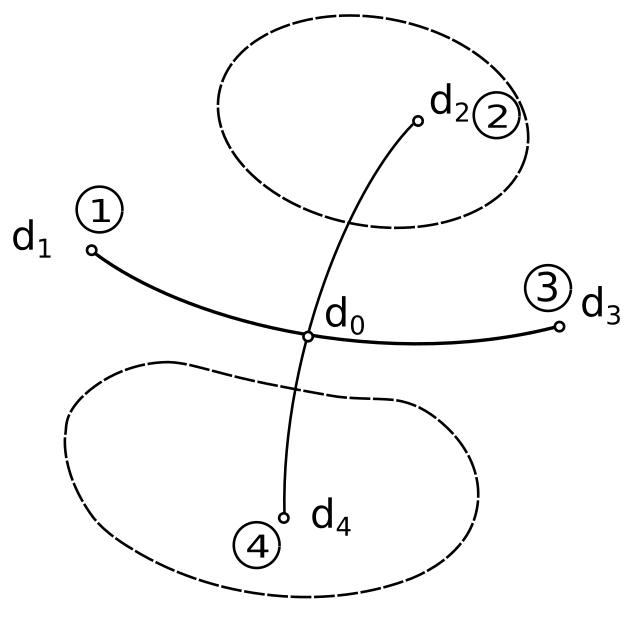
\includegraphics[scale=0.3]{drawing}
\end{figure}

Şekil 4.5.3 Durum 1' in incelenmesi.\\[0.1in]
Teorem 4.5.1' in tanıtlanmasında izlediğimiz yolun
benzeri biçimde,
\begin{equation*}
	Ç_1 = Ç - (d_0)
\end{equation*}
\end{document}
